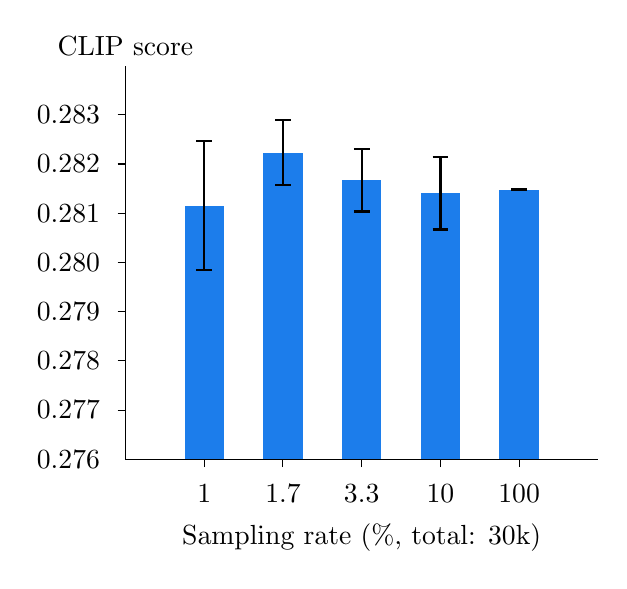
\begin{tikzpicture}
    \definecolor{plot_blue}{RGB}{28,125,235}
    % axis
    \draw (0,0) -- (6,0);
    \draw (0,0) -- (0,5) node[above] {CLIP score};

    % transform equaition from real value for plotting
    % 5 * (x - 0.276) / 0.008

    \foreach \y/\value in {0/0.276, 0.625/0.277, 1.25/0.278, 1.875/0.279, 2.5/0.280, 3.125/0.281, 3.75/0.282, 4.375/0.283} {
        \node[left] at (-0.2, \y) {\value};
    }

    \foreach \c in {1, 2, 3, 4, 5, 6, 7}{
        \draw (-0.1, {({\c}*0.625)}) -- (0, {({\c}*0.625)});
    }

    % label of x-axis
    \foreach \x/\label in {1/1, 2/1.7, 3/3.3, 4/10, 5/100} {
        \draw ({\x},-0.1) -- ({\x},0.1);
        \node[below] at ({\x},-0.2) {\label};
    }

    \node[below] at (3, -0.7) {Sampling rate (\%, total: 30k)};
    
    % bar
    \fill[plot_blue] (0.75, 0) rectangle (1.25, 3.223);
    \fill[plot_blue] (1.75, 0) rectangle (2.25, 3.893);
    \fill[plot_blue] (2.75, 0) rectangle (3.25, 3.542);
    \fill[plot_blue] (3.75, 0) rectangle (4.25, 3.377);
    \fill[plot_blue] (4.75, 0) rectangle (5.25, 3.425);
    
    % error bar
    \draw[thick] (1, 2.40125) -- (1, 4.04625);
    \draw[thick] (0.9, 2.40125) -- (1.1, 2.40125);
    \draw[thick] (0.9, 4.04625) -- (1.1, 4.04625);

    \draw[thick] (2, 3.47875) -- (2, 4.30875);
    \draw[thick] (1.9, 3.47875) -- (2.1, 3.47875);
    \draw[thick] (1.9, 4.30875) -- (2.1, 4.30875);

    \draw[thick] (3, 3.148125) -- (3, 3.935625);
    \draw[thick] (2.9, 3.148125) -- (3.1, 3.148125);
    \draw[thick] (2.9, 3.935625) -- (3.1, 3.935625);

    \draw[thick] (4, 2.91875) -- (4, 3.835);
    \draw[thick] (3.9, 2.91875) -- (4.1, 2.91875);
    \draw[thick] (3.9, 3.835) -- (4.1, 3.835);

    \draw[thick] (5, 3.425) -- (5, 3.425);
    \draw[thick] (4.9, 3.425) -- (5.1, 3.425);
    \draw[thick] (4.9, 3.425) -- (5.1, 3.425);

\end{tikzpicture}
